% Chapter 2: System Requirements and Architecture
\chapter{System Requirements and Architecture}

The successful development of such an application requires meticulously defined set of requirements and a robust architectural design. For a system that requires accurate real-world data, precise measurements of fixtures, comprehensive database of products with precise measurements and business logic that gets used while selection process of a shower enclosure, this foundation phase is particularly critical. It ensures the implementation is not only technologically sound but also directly aligned with the user needs and business objectives.

The transition from a conceptual framework to a functional software requires a systematic approach to defining the system's intended behavior, constraints, and underlying structure. This chapter delineates the complete process of designing the LiDAR-based product recommendation system, beginning with a thorough analysis of functional and non functional requirements.

Following the requirement analysis, a review of the current state of the art in indoor scanning, 3d point cloud data processing, and configuration recommendation engines are presented. this review critically evaluates existing solutions and methodologies, thereby contextualizing the novel approach taken in this thesis. The chapter then transitions from the what to the how, presenting a detailed system architecture and justifying the chose of the technology stack. Finally, the chapter concludes with the logical data model design, providing a blueprint for how information is structured, stored and accessed within the PostgreSQL database, which serves as the backbone of the system's data-driven logic.

\section{Requirement Analysis}

This section outlines the analysis of the existing system's shortcomings and defines the functional and non-functional requirements for the new product recommendation system.

\subsection{Problem Statement and Background}

An analysis of the company's internal processes revealed significant inefficiencies in the existing workflow for generating quotes for shower enclosures. These challenges stem from the limitations of previously used software solutions.

\subsubsection{Challenges with Legacy Commercial Software}

The primary software used for quote generation was "HERO Software"\cite{AlleFeaturesHERO}, a comprehensive but overly complex tool for the company's specific needs. Based on feedback from the sales department, two main issues were identified:

\begin{enumerate}
    \item \textbf{High Usability Barriers}: The software's interface was not intuitive for sales personnel, often requiring intervention from the IT department to configure quote templates and calculation parameters.(add footnote reference review from sales team)
    \item \textbf{Requirement of Expert Knowledge}: Effective use of the software's configurator demanded deep expertise in construction details (e.g., gutter placement, faucet location). This dependency led to a steep learning curve and a high probability of errors, especially for new employees.
\end{enumerate}

Furthermore, the software's high licensing costs posed a significant financial burden, especially since many of its features, designed for general construction, were rarely used by the company.

\subsubsection{Limitations of the Subsequent In-House Solution}

To address these issues, a simpler, more user-friendly application called "Angeboteskonfigurator" or "Offer Configurator" was developed internally using JavaScript. While this application improved usability, it introduced a different problem: it lacked intelligent filtering capabilities. The sales team still could not automatically select or recommend shower enclosures based on critical parameters such as:

\begin{itemize}
    \item Dimensions (width, depth, height)
    \item Shower construction style (e.g., niche, corner entry, walk-in)
    \item Door type (e.g., folding, sliding, pivot)
    \item Orientation (left, right, or universal)
\end{itemize}

This lack of intelligent logic meant the process was still manual and prone to selection errors.

\subsubsection{Limitations of the Partner's database}

The partner's database functioned as a business-to-business (B2B) website, supplying the company with discounted products across the home renovation spectrum, including shower enclosures and other bathroom-related items. A critical deficiency was the lack of an Application Programming Interface (API), which prevented programmatic access to product data for shower enclosures or other fixtures.

Although the website offered a configurator, developed by the manufacturer of the product line, that could suggest shower enclosures based on width and depth, its usability was hampered by a cumbersome navigation requiring multiple clicks to specify the desired shower type and opening mechanism. Moreover, the configurator presented an incomplete range of options, omitting several configurations that were explicitly detailed in the product catalog. While a wide array of style choices was available—such as various glass types, profile colors, anti-water coatings, automatic close features, and profile styles—internal company reviews highlighted a preference for the most basic designs, a preference driven primarily by the insurance-funded customer base.

\subsubsection{Traditional Sales Process}

The company's most traditional sales process was rudimentary and highly manual, relying on a six-page A4-sized printed questionnaire and product selector during initial customer consultations. This document, which lacked product images and only listed basic shower and door types, was the source of significant operational inefficiency.

The workflow required sales staff to manually transcribe customer requirements from the paper form into a digital configurator. Subsequently, they had to select a suitable shower enclosure while performing multi-step calculations to align the final price with the customer's budget. This involved accounting for the company's profit margin, which is primarily derived from the material price of shower enclosures, making the calculation both critical and prone to error. The process was cumbersome and inefficient, significantly increasing the time required to generate accurate quote.

\subsection{System Requirements}

Based on the analysis of the existing problems, the following functional and non-functional requirements have been defined for the new system.

\subsubsection{Functional Requirements}

The system must provide the following functionalities:

\begin{table}[h]
\centering
\caption{Functional Requirements}
\label{tab:functional_req}
\begin{tabular}{|l|p{0.6\textwidth}|l|}
\hline
\textbf{ID} & \textbf{Requirement} & \textbf{Priority} \\
\hline
FR-1 & The system shall allow users to input shower dimensions (width, depth, height) to filter compatible products. & Must-have \\
\hline
FR-2 & The system shall enable filtering of shower enclosures by construction style (e.g., niche, corner, U-shape). & Must-have \\
\hline
FR-3 & The system shall allow filtering of products by door type (e.g., sliding, pivot, folding). & Must-have \\
\hline
FR-4 & The system shall allow filtering by shower door orientation (left, right, or universal). & Should-have \\
\hline
FR-5 & The system shall generate a preliminary quote based on the selected product and configuration. & Should-have \\
\hline
FR-6 & The system shall be fully compatible with the macOS operating system. & Must-have \\
\hline
FR-7 & The system shall provide a documented API to allow for programmatic searching of compatible products. & Must-have \\
\hline
FR-8 & The system shall include an administrative back-end for managing the product catalogue (CRUD). & Must-have \\
\hline
FR-9 & The system shall include an administrative back-end for managing user accounts (CRUD). & Must-have \\
\hline
FR-10 & The system shall provide a dashboard displaying key usage statistics. & Nice-to-have \\
\hline
FR-11 & The system shall automatically synchronize product pricing from the partner's data source. & Nice-to-have \\
\hline
\end{tabular}
\end{table}

\subsubsection{Non-Functional Requirements}

The system must adhere to the following quality attributes:

\begin{table}[h]
\centering
\caption{Non-Functional Requirements}
\label{tab:non_functional_req}
\begin{tabular}{|l|p{0.6\textwidth}|l|}
\hline
\textbf{ID} & \textbf{Requirement} & \textbf{Priority} \\
\hline
NFR-1 & The user interface shall be highly intuitive, requiring minimal training for non-technical sales staff. & Must-have \\
\hline
NFR-2 & The system shall generate product recommendations in under 3 seconds to enable real-time consultations. & Must-have \\
\hline
NFR-3 & The system's UI shall be responsive and fully functional on both desktop and tablet devices. & Should-have \\
\hline
NFR-4 & The total cost of ownership (TCO) shall be significantly lower than the previously licensed software. & Must-have \\
\hline
NFR-5 & The system shall be architected to support multi-lingual user interfaces (internationalization, i18n). & Should-have \\
\hline
NFR-6 & The system's database shall be backed up automatically on a daily schedule. & Nice-to-have \\
\hline
\end{tabular}
\end{table}

\section{State of the Art and Approach}

This section reviews the state-of-the-art in technologies relevant to this thesis, beginning with an analysis of LiDAR scanning applications for interior mapping. It then examines existing product recommendation and configuration systems to identify the current technological gaps, and finally, outlines the methodological approach adopted to address these gaps. The review begins with LiDAR technology, which was initially developed for terrain mapping in aeronautics and aerospace applications. It has since expanded into diverse domains such as autonomous vehicles, enabling these systems to navigate their environments effectively and generate three-dimensional imagery that can be transformed into Building Information Modeling (BIM) or Computer-Aided Design (CAD) models. \cite{waykarLidarTechnologyComprehensive2022a}

\subsection{Introduction of LiDAR in edge devices}

Owing to significant advances in laser diode technology, optics, and manufacturing, LiDAR systems have become smaller, more accessible, and cost-effective \cite{waykarLidarTechnologyComprehensive2022a}. This miniaturization has paved the way for the integration of LiDAR into edge devices, a trend most prominently exemplified by its inclusion in consumer smartphones like the Apple iPhone Pro series and iPad Pro series. The presence of LiDAR in these devices has significantly broadened public access to sophisticated spatial scanning capabilities.

A variety of mobile applications have emerged to leverage these on-device sensors, including PolyCam, LumoScanner, and MagicPlan. Notably, such applications often existed prior to the integration of built-in LiDAR, previously relying on external, Bluetooth-enabled laser range finders for high-accuracy data capture. A comparative study of several of these scanning solutions provides strong academic validation for the choice of MagicPlan in this thesis. The study concluded that MagicPlan was the most effective and efficient method for as-built modeling, highlighting its superior performance in functionality, usability, and processing speed (9.02 m²/min) and awarding it the highest overall score of 4.26. These findings affirm that the company's incumbent tool is a robust and well-founded choice for the data acquisition phase of this project. \cite{mortazaviEvaluatingSiteScanning2024a}

The LiDAR sensor, optimized for room scanning, measures distances up to 5 meters. However, its full potential is realized only when paired with sophisticated software applications like MagicPlan. By combining augmented reality (AR) with artificial intelligence (AI), MagicPlan automatically detects and classifies objects, capturing a scene's complete geometry beyond basic features like floors or walls. A LiDAR-derived room scan, where data is recorded, identified, and processed by AI, holds significant long-term value as the information remains accessible and reusable \cite{geibWhyApplesLiDAR}.

These sensors enable the creation of precise three-dimensional visualizations through dense point cloud data, providing valuable spatial information. MagicPlan's proprietary processing software employs advanced algorithms and AI models to convert these visualizations into editable CAD models. While specific technical details and proprietary algorithms are not publicly disclosed, MagicPlan's integration with Apple's RoomPlan API suggests a hybrid approach, combining AI-driven spatial recognition with sensor data processing for classifying and mapping interior objects \cite{geibWhyApplesLiDAR}.

The improved LiDAR scanner in devices like the iPad Pro and iPhone 12 Pro, coupled with specialized floor plan applications, significantly enhances accuracy in room dimensions and allows for the inclusion of richer detail in floor plans \cite{geibWhyApplesLiDAR}. This integration facilitates advanced visualization, web-based uploading of 2D floor plans and 3D models, and seamless information sharing. Critically, this technology can boost client acquisition through innovative engagement, serve as a basis for rapid material and cost estimates during initial site visits, and bolster quality assurance by enabling comparisons of renovation stages. The capacity to proactively detect errors and compare planned versus actual progress positions LiDAR room scans as invaluable, cost-saving roadmaps within the residential construction sector \cite{geibWhyApplesLiDAR}.  

\subsection{Analysis of the Incumbent Product Configurator}

While MagicPlan addresses spatial data acquisition, the second component of the established workflow is a manufacturer-provided, web-based product configurator. This section provides a state-of-the-art analysis of this incumbent tool, identifying the specific technical and functional limitations that are the root cause of the business and operational inefficiencies outlined in the Problem Statement. This tool, hosted on a B2B wholesale portal, is the primary instrument for specifying and ordering compatible shower enclosure components.

The configurator guides users through a hierarchical selection process to ensure component compatibility. It allows for the definition of several key parameters, such as:
\begin{itemize}
    \item \textbf{Entry Type:} Including corner shower (\textit{Ecklösung}), alcove shower (\textit{Nischenlösung}), walk-in shower (only 1 side-panel / door other side empty), and U-form configurations(multiple options 1 door 2 sidepanel, 2 doors, 1 sidepanel, 2 doors 2 sidepanels, half-circle(not-used)).
    \item \textbf{Shower Style:} Such as a corner cabin (\textit{Eckkabine}) or a corner entry with a full or shortened side panel (Only when there is a short sidewall present or a bathtub is beside the shower).
    \item \textbf{Door Type:} Options include swing doors (\textit{Pendeltür}), folding swing doors (\textit{Faltpendeltür}), and sliding doors (\textit{Gleittür}).
    \item \textbf{Installation Details:} Including orientation and mounting type (floor-level or on a shower tray).
\end{itemize}

Based on these initial selections, the system subsequently recommends compatible components like side panels or doors. For these components, it provides critical dimensional data, including the minimum (\textit{minEinbau}) and maximum (\textit{maxEinbau}) construction range.

Despite its function in ensuring hardware compatibility, a critical analysis of the configurator reveals significant operational and technical limitations that justify the development of a new, integrated solution:

\begin{enumerate}
    \item \textbf{Lack of Real-Time Price Visibility:} The system does not display component pricing during the configuration process. Prices are only revealed after a product is added to the shopping cart. This limitation severely hampers the sales team, who must select products to fit a customer's budget after a partial quote has already been generated. The issue is exacerbated by a functional limit of thirteen shopping carts per user, which are reportedly always at full capacity.
    \item \textbf{Limited Product Options:} For any given selection, the configurator presents only a single product line, precluding the comparison of alternative products or styles that might be available.
    \item \textbf{B2B Exclusivity and Price Opacity:} As a wholesale portal, the platform is inaccessible to end-customers and displays the company's net acquisition costs. This lack of transparency makes it unsuitable for direct use in client consultations.
    \item \textbf{Outdated Product Data:} The configurator frequently omits new product configurations that are present in the manufacturer's official product catalog and even on the consumer-facing website. Accessing these newer options depends on an employee's specialized knowledge of the print catalog, creating a significant knowledge barrier for new hires and increasing the likelihood of suboptimal product selections.
    \item \textbf{No Integration Capabilities:} The tool is a standalone, closed system with no capacity for integration with external applications like MagicPlan. This results in a fragmented workflow that requires manual and error-prone data transfer from the room scan to the product configurator.
    \item \textbf{Closed Architecture:} The platform does not offer Application Programming Interfaces (APIs) for accessing its product database, configuration logic, or cart system. This fundamentally prevents automation, data synchronization, or integration with other business-critical software.
    \item \textbf{Lack of Shower Tray Recommendation:} While the configurator prompts the user to select an installation type (with or without a shower tray), it does not subsequently recommend a compatible shower tray product. This omission creates an incomplete solution for a full shower replacement, forcing sales staff to manually identify and verify a suitable tray from a separate catalog. This represents a significant gap in providing a comprehensive and seamless customer solution.
\end{enumerate}

In summary, the configurator's closed architecture, outdated data, and inefficient workflow are the direct technical sources of the operational bottlenecks, financial risks, and sub-optimal customer experiences described in the problem statement. This analysis proves that a significant technological gap exists, justifying the development of the modern, integrated, and intelligent product recommendation system proposed by this thesis.

The preceding analysis demonstrates that while powerful tools for spatial scanning and product configuration exist, they operate in isolation. This thesis addresses this critical gap.

Based on an evaluation of the available technologies, this project will utilize the MagicPlan application and its API for data acquisition and take data, configurator from the wholesale website. Subsequent chapters will provide a detailed account of the data processing methods and their application within the product recommendation algorithm.

\section{System Architecture and Technology Stack}

To address the critical limitations of the incumbent product configurator identified in Section 2.2.2—namely its closed architecture, lack of integration capabilities, and outdated data—this thesis proposes a modern three-tier system architecture. This design is explicitly engineered to provide real-time data integration, a flexible and open API, and automated data synchronization, directly solving the previously discussed operational bottlenecks. The architectural pattern separates the system into presentation, application, and data layers, enabling modularity, scalability, and maintainability.

\subsection{Architectural Design and Rationale}

The system is structured into three distinct tiers, as illustrated in Figure \ref{fig:three-tier-architecture}. This separation allows each tier to be developed, scaled, and maintained independently.

\begin{figure}[h]
\centering
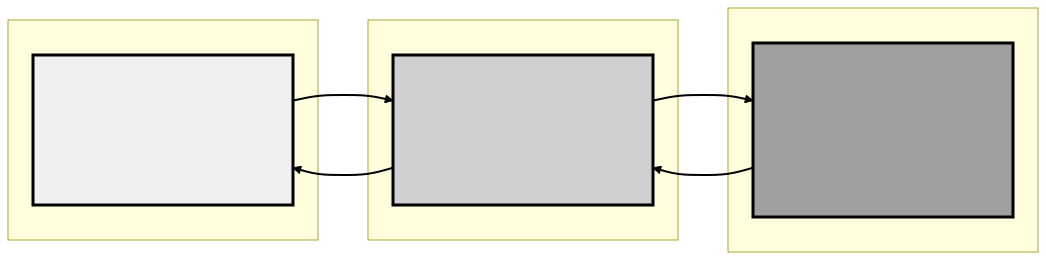
\includegraphics[width=0.8\textwidth]{2_Sources/Assets/Chapter2/three-tier-architecture.png}
\caption{Three-Tier System Architecture}
\label{fig:three-tier-architecture}
\end{figure}

\textbf{The Presentation Tier (Frontend):} This tier is responsible for the user interface and client-side experience. It directly addresses the "B2B Exclusivity" and poor usability of the old configurator by providing a modern, responsive interface suitable for direct use in client consultations.
\begin{itemize}
    \item \textbf{Key Responsibilities:} Rendering product recommendations, visualizing room layouts from MagicPlan data, and capturing user inputs for configuration.
    \item \textbf{Technology:} Next.js with TypeScript.
\end{itemize}

\textbf{The Application Tier (Backend):} This tier acts as the central nervous system of the application, directly solving the "No Integration Capabilities" and "Closed Architecture" problems of the incumbent system. It serves as an integration hub, decoupling the frontend from the data sources and external services.
\begin{itemize}
    \item \textbf{Key Responsibilities:}
    \begin{itemize}
        \item Exposing a secure, well-documented RESTful API to be consumed by the frontend client and other authorized third-party applications.
        \item Handling user authentication and authorization to support multi-user access.
        \item Consuming room dimension and fixture data from the MagicPlan API.
        \item Executing the core business logic for product matching, which primarily employs rule-based and graph-based recommendation algorithms (rather than machine learning models), complemented by advanced search logic, such as suggesting dimensionally-adjusted alternatives when no products meet an initial price constraint.
        \item Implementing the logic for ancillary product recommendations, such as compatible shower trays, to solve the "Lack of Shower Tray Recommendation" gap.
        \item Orchestrating automated data-sourcing tasks.
        \item Use of NLP search, where the user just need to write the type of shower they need with or without dimensions and price range, and they are shown a product based on the input.
    \end{itemize}
    \item \textbf{Technology:} Express.js with TypeScript, with Python for specialized automation scripts.
\end{itemize}

\textbf{The Data Tier (Database):} This tier provides a single source of truth for all application data, ensuring integrity and eliminating the data fragmentation and staleness issues of the previous workflow.
\begin{itemize}
    \item \textbf{Key Responsibilities:} Persistently storing the full product catalog, complex component compatibility rules, processed MagicPlan scan data, and user information.
    \item \textbf{Technology:} PostgreSQL.
\end{itemize}

\subsection{Technology Stack Justification}

The technological stack was chosen to provide a reliable, up-to-date, and maintainable application that directly addresses the shortcomings of the previous system.

\begin{itemize}
    \item \textbf{Frontend (Next.js \& TypeScript):} Next.js, a React framework, was chosen for its capabilities in server-side rendering (SSR) and static site generation (SSG), ensuring high performance and a professional user experience. Its component-based architecture is ideal for building a complex product configurator. TypeScript adds static typing, which is crucial for maintaining a large codebase and ensuring clear data contracts with the API, reducing runtime errors.
    \item \textbf{Backend (Express.js \& TypeScript):} To provide the adaptable and potent RESTful API that the existing system lacked, Express.js, a simple web framework for Node.js, was chosen. Because of its unbiased nature, the API structure can be specifically designed to meet the objectives of this project. For the API endpoints, TypeScript guarantees consistency and concise documentation.
    \item \textbf{Database (PostgreSQL):} PostgreSQL, an open-source object-relational database system (ORDBMS), was selected due to its resilience, ACID compliance, and dependable support for complex queries and data interactions \cite{makrisMongoDBVsPostgreSQL2021}. This is necessary to enable features like shower tray recommendations and to mimic the complex compatibility requirements between various shower enclosure components (doors, side panels, etc.).
    \item \textbf{Automation (Python):} Because Python has a large ecosystem of libraries for data manipulation and web scraping (like Selenium), it was chosen for the backend automation and data scraping chores. By maintaining the product catalog and pricing data up to date, this option immediately supports the automated jobs that address the "Outdated Product Data" and "No Real-Time Price Visibility" issues.
    \item \textbf{Containerization (Docker):} The entire application stack is containerized using Docker. This reduces the risks associated with inconsistent environments and streamlines the deployment process by maintaining a constant environment throughout development, testing, and deployment.
\end{itemize}

\subsection{Data Flow and Automation}

The architecture is designed to support a seamless flow of data, from initial room scan to final product recommendation.

\begin{enumerate}
    \item \textbf{Data Acquisition:} A user performs a room scan using the MagicPlan app. The dimensional and fixture data is retrieved via an API call from the Application Tier.
    \item \textbf{Processing \& Logic:} The Application Tier extracts key measurements from the processed spatial data, such as the dimensions of existing fixtures. The recommendation engine then queries the PostgreSQL database for compatible products based on the room's constraints and the system's embedded compatibility rules.
    \item \textbf{Recommendation:} A curated list of suitable products is sent to the Presentation Tier and displayed to the user for final selection. This API-centric approach has already proven its value, as the backend is currently being used by the company's proprietary quote-generation software to retrieve curated product lists, demonstrating the flexibility that was absent in the previous system.
\end{enumerate}

To ensure data is always current, two primary automated background jobs run on the backend:
\begin{itemize}
    \item \textbf{Product Ingestion Service:} A Python script that can ingest new product data from manufacturer sources, populating the PostgreSQL database and keeping the product catalog complete.
    \item \textbf{Price Update Service:} A Python script that periodically scrapes partner portals to update pricing for existing products in the database, ensuring that all quotes are based on real-time data.
\end{itemize}

This automated, API-driven architecture stands in stark contrast to the manual, fragmented, and error-prone workflow of the incumbent system.

\section{Data Model Design}

The product recommendation system's accuracy, performance, and future scalability are all directly impacted by a solid and scalable data model \cite{10.1145/331983.331984}. The PostgreSQL database schema, which is designed to effectively process and store complex spatial data from LiDAR scans, manage a multifaceted product catalog, store user data for authentication, complex product relationships, and customer data for automation, is described in detail in this section. The main objective is to develop a logical framework that makes it easier to do the intricate queries needed by the rule-based and graph-based recommendation algorithms.

PostgreSQL was selected over MongoDB primarily because of its superior response time, which is essential when querying for a combination in products database; its ability to reduce overall dataset storage size, which is crucial for lowering hosting service costs for the company; and its reliable and automated backup management, which is offered as an option with many well-known hosting services. \cite{makrisMongoDBVsPostgreSQL2021}

\subsection{Core Data Entities and Their Relationships}

The data model is structured around a set of core entities that create a logical division between user data, spatial information from scans, and the product catalog. This architectural choice is crucial for maintaining data integrity, enabling scalability, and optimizing query performance. The foundational entities are:

\begin{itemize}
    \item \textbf{User:} Represents an authenticated system operator. This entity holds credentials and role-based access control information (via the \texttt{isAdmin} flag), linking users to the plans and products they create. It is also crucial for managing concurrent usage across multiple users.
    \item \textbf{Plan:} The \texttt{Plan} entity is structured to encapsulate a complete project scanned via the MagicPlan app. It serves as the top-level container for a specific customer's quote request, linked to a company \texttt{User} who created it. This design is crucial for associating the customer with the \texttt{Rooms} within the plan and for storing essential customer-related metadata (such as customer name and ID) and a thumbnail URL for UI representation.
    \item \textbf{Room:} Represents a distinct spatial area within a \texttt{Plan}. It stores dimensional data (e.g., \texttt{areaWithInteriorWalls}) and serves as a container for all \texttt{Fixture} objects identified within its boundaries. This entity is crucial for filtering to specific contexts, such as bathrooms.
    \item \textbf{Fixture:} Models a fixed installation or obstacle (e.g., window, door, existing bathtub) within a \texttt{Room}. Each fixture's dimensions and location are critical inputs for the recommendation algorithm, as they impose physical constraints on product placement.
    \item \textbf{Product:} The foundational entity of the product catalog. It represents a core, purchasable item (e.g., a specific model of shower door, tray) and contains universal attributes like \texttt{modelNumber}, price, and base dimensions. It is linked to a \texttt{ProductType} for categorization.
    \item \textbf{ProductType:} Provides a categorical framework for the product catalog (e.g., "Shower Door," "Side Panel," "Shower Tray"). This entity allows for logical grouping, filtering, and ensures the system is extensible to future product categories.
    \item \textbf{Product-Specific Details (\texttt{DoorDetail}, \texttt{ShowerCabinDetail}, \texttt{ShowerTrayDetail}):} These entities are linked to the \texttt{Product} table via a one-to-one relationship. This architectural pattern avoids a bloated and sparse \texttt{Product} table by abstracting type-specific attributes (like \texttt{openingType} for a door or \texttt{style} for a cabin) into separate, specialized tables.
    \item \textbf{ProductRelationship:} This is the most critical entity for the recommendation logic. It functions as a "join table" that connects two \texttt{Product} entities (\texttt{sourceProduct} and \texttt{targetProduct}), defining a specific \texttt{RelationshipType} between them. This structure effectively transforms the product catalog into a directed graph, where products are nodes and compatibility rules are the edges—the essential foundation for the graph-based algorithm.
\end{itemize}

\begin{figure}[h]
\centering
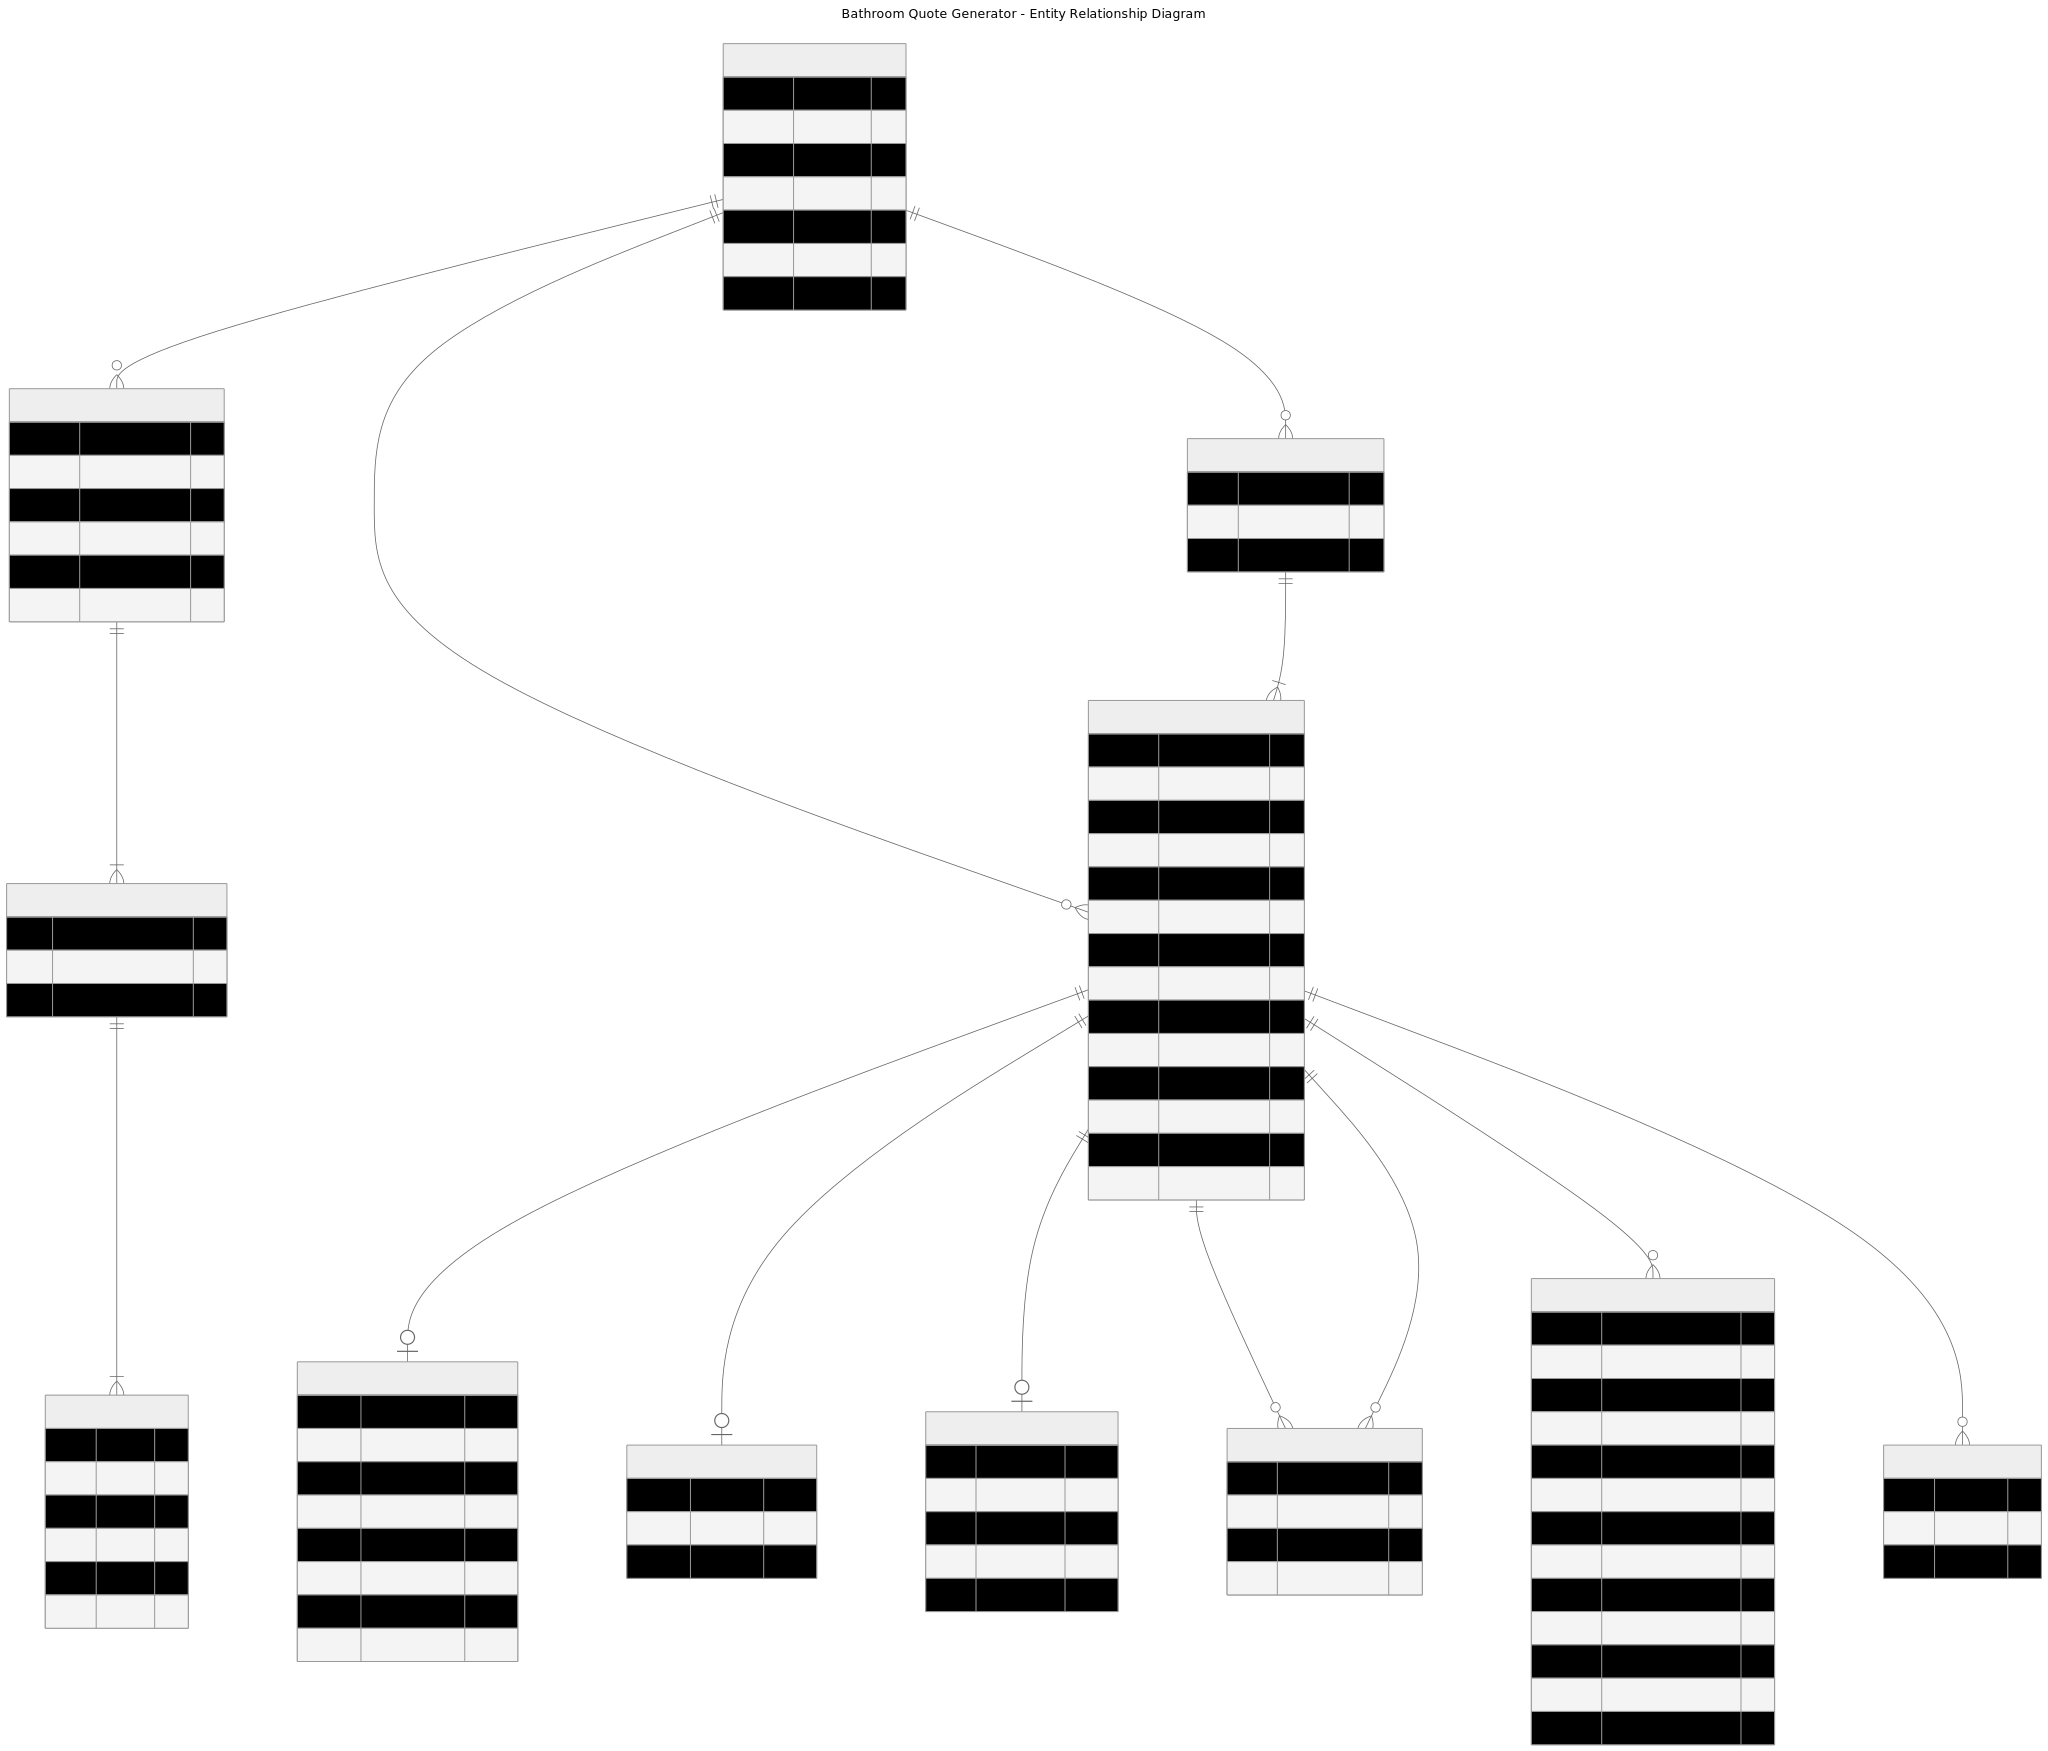
\includegraphics[width=0.8\textwidth]{2_Sources/Assets/Chapter2/thesis-er-diagram.png}
\caption{Entity-Relationship Diagram of the Database Schema}
\label{fig:er-diagram}
\end{figure}

\subsection{Architectural Justification and Scalability}

The schema is intentionally designed to be both robust and extensible. The separation of the \texttt{Product} entity from its type-specific details (\texttt{DoorDetail}, etc.) is a key example of normalization. This pattern ensures that the core \texttt{Product} table remains lean, while allowing for immense flexibility in defining attributes for new product types without requiring disruptive schema changes.

Furthermore, the design for scalability is most evident in the \texttt{ProductRelationship} model. By representing compatibility as explicit relationships in a dedicated table, the system can:
\begin{enumerate}
    \item \textbf{Scale to new compatibility rules:} Adding new relationship types (e.g., \texttt{REQUIRES\_SCREWS}, \texttt{ACCESSORY\_FOR}) can be achieved by simply adding a new value to the \texttt{RelationshipType} enum.
    \item \textbf{Support complex, graph-based queries:} The model is optimized for algorithms that traverse the product graph to find valid combinations, which is far more efficient and powerful than embedding such logic in application code.
    \item \textbf{Accommodate new product styles:} When a new product is added, its compatibility with the existing ecosystem is defined simply by inserting new rows into the \texttt{ProductRelationship} table, seamlessly integrating it into the recommendation engine.
\end{enumerate}

This graph-based data architecture, combined with the normalized structure, provides a powerful and future-proof foundation for the intelligent recommendation system.

\section{Future Developments and Scalability Opportunities}

The application is built with technologies that scale well with changes. It is under constant development and it is possible to improve the suggested system even further. The improvements foreseen in the future of Rule based shower configuration selection are:

\subsection{Intelligent Shower Type Recommendation Based on User History}

Currently, the system enables users to manually select shower configurations based on their requirements. However, a more advanced version could implement automated recommendations by analyzing previous selections and applying rule-based logic \cite{mangiliBayesianApproachConversational2020}. This enhancement would consider the following factors:

\begin{itemize}
    \item The customer's preference to transition from old shower to new shower
    \item Dimensional and location consistency with previously selected showers
    \item Customer preference for enclosure updates without fixture replacement
\end{itemize}

Based on these criteria, the system could perform spatial analysis to evaluate the available space in front of the shower and identify any obstacles or connected fixtures such as bathtubs. This information would enable the recommendation of appropriate door opening mechanisms. For instance, if a toilet is positioned 30 cm from the shower entrance, the system could suggest sliding doors to accommodate the spatial constraints. Alternatively, for locations with limited clearance on both sides, pivot doors that open both inward and outward could be recommended to prevent collision issues while maintaining functionality.

\subsection{Comprehensive Bathroom Renovation Module Using Artificial Intelligence}

The current implementation focuses exclusively on shower enclosure selection within specified dimensions. However, the system can be expanded to include additional bathroom fixtures and materials, such as toilets, wash basins, grab handles, faucets, wall coverings, tiles, folding seats, and thermostats. This expansion would enhance profitability by offering more comprehensive solutions to customers.

The existing relationship model can be extended to maintain product compatibility across categories. For example, toilets can be linked with appropriate flush systems based on installation type (wall-mounted or concealed), and wash basins can be paired with compatible faucets. This prevents accidental selection of incompatible products.

Artificial intelligence could further personalize recommendations by incorporating additional customer information, such as age, insurance coverage status, and mobility requirements. This data would allow the system to filter available options accordingly. For instance, elderly customers or those with mobility limitations could be presented with grab handles, folding seats, and walk-in shower configurations designed for accessibility.

\subsection{Machine Learning-Based Bathroom Layout Optimization}

The current spatial analysis approach could be enhanced through machine learning techniques trained on multiple floor plans. With sufficient training data, the system could predict optimal fixture placement within bathroom spaces or employ reinforcement learning methods that reward effective spatial arrangements \cite{diDeepReinforcementLearning2021}.

However, this approach faces several limitations. Bathroom designs vary significantly across buildings due to structural differences, making training effective only for homogeneous datasets where variations are limited to room size, door position, and window location \cite{diDeepReinforcementLearning2021}. Additionally, the data provided by floor plan APIs often presents preprocessing challenges. Specifically, the API returns coordinates for external walls but not internal walls, and fixtures are represented by a single center point and dimensions, creating significant data misalignment that requires extensive preparation before analysis can begin.

Furthermore, the floor plan software sometimes produces inaccurate results—such as placing fixtures outside the defined room boundaries without creating appropriate enclosures, or failing to correctly align walls to 90-degree angles despite the actual measurements being perpendicular. These technical limitations must be addressed before this enhancement can be reliably implemented.

\subsection{Visual Previews via Generative AI and Diffusion Models}

Currently there are two popular approaches for image generation and image editing: Generative Adversarial Networks \cite{goodfellowGenerativeAdversarialNets2014} and Diffusion Models \cite{hoDenoisingDiffusionProbabilistic2020}. Furthermore, Diffusion models for their capacity to generate high quality, photorealistic images. Their effective integration with Large Language Models (LLMs) also facilitates the straightforward translation of a user's textual ideas into visual concepts, as demonstrated by systems like VIDES \cite{leVIDESVirtualInterior2023}.

Diffusion models with editing capabilities could enable customers to visualize proposed bathroom designs by processing photographs taken at appropriate angles. However, two significant practical barriers currently prevent its deployment. First, a primary challenge lies in workflow integration. The existing system is optimized for rapid, automated quote generation. Introducing a manual step, such as requiring user input to select a specific area in an image, would add latency and hinder this core function. This suggests the feature might be better suited for optional, high-end design services rather than for immediate quoting.

Second, a more fundamental technical barrier is data scarcity. The product database contains limited visual assets—typically only one or two promotional images and basic CAD-style line drawings per product. This lack of diverse, high-fidelity imagery would severely challenge the ability of any generative model to produce varied and realistic renderings of the products within a new scene.

\subsection{Intelligent Chatbot Assistant for Budget-Conscious Recommendations}

A chatbot interface could provide intelligent suggestions when a recommended shower configuration exceeds the customer's budget. The system could strategically suggest modifications—such as reducing width or depth—while maintaining aesthetic coherence and functionality. This would help customers find solutions that balance their financial constraints with their design preferences \cite{sunConversationalRecommenderSystem2018}.
